\documentclass[oneside]{VUMIFPSkursinis}
\usepackage{algorithmicx}
\usepackage{algorithm}
\usepackage{algpseudocode}
\usepackage{amsfonts}
\usepackage{float}
\usepackage{amsmath}
\usepackage{bm}
\usepackage{caption}
\usepackage{color}
\usepackage{float}
\usepackage{graphicx}
\usepackage{listings}
\usepackage{subfig}
\usepackage{tabularx}
\usepackage{wrapfig}
\newcolumntype{P}[1]{>{\centering\arraybackslash}p{#1}}
\usepackage[%  
    colorlinks=true,
    linkcolor=black
]{hyperref}
\university{Vilniaus universitetas}
\faculty{Matematikos ir informatikos fakultetas}
\department{Programų sistemų katedra}
\papertype{Programų sistemų inžinerija II laboratorinis darbas I}
\title{Reikalavimų apibrėžimas}
\titleineng{Requirements specification}
\status{2 kurso 3 grupės studentai}
\secondauthor{Justas Tvarijonas}  
\thirdauthor{Greta Pyrantaitė}
\fourthauthor{Rytautas Kvašinskas}
\author{Tomas Kiziela}

\supervisor{Audronė Lupeikienė, M. Darbuot., Dr.}
\date{Vilnius – \the\year}


\bibliography{bibliografija}

\begin{document}
\maketitle
\tableofcontents

\section{Įžanga}
Mūsų komanda gavo kitos komandos pirmame semestre(PSI I) paruoštą slidinėjimo kurorto projektą. Šiame darbe sieksime toliau plėtoti ir keisti šį projektą. Toliau vystatnt projektą keisis daugumas dalių. Siekiant padaryti gerą produktą kai kurios  dalys bus pašalindos ir pridėtos naujos. Pirmame semestre projektuojant dėmesys buvo skiriamas klasikinei projektavimo paradigmai. Šiame darbe projektą rašysime pasinaudodami ICONIX principu, projektuojant dėmesys bus skiriamas GUI sudarymo ir iš to išplauks sistemos projektavimas ir sandara. 

\section{Reikalavimai}
Šioje dalyje bus pateikti funkciniai bei nefunkciniai reikalavimai sistemai. Stengsimės prisilaikyti ,,užsakovų"(grupės iš kurios gavome jų darbą) reikalavimus tačiau siekiant sukurti geresnę sistemą pridėsime kaikuriuos savo sugalvotus reikalavimus arba ignoruosime mums pateiktus reikalavimus. 

\subsection{Reikalavimų pataisymai}
	\begin{itemize}
		\item{X - ištrintas}
		\item{M - pakeistas}
	\end{itemize}


\begin{table}[htbp]


\begin{tabularx}{1\textwidth}{  |P{1cm}|X|P{1.5cm}|p{3.5cm}|X| }  \hline
	Nr. & Pradiniai reikalavimas&  Pakeitimo tipas & Klaidos aprašas  & Naujas reikalavimas \\ \hline
	FR & ,,Žetonas" seka vartotojo laiką praleistą trasoje & M & Pakeistas neaiškus daiktavardis & Sekimo prietaisas seka vartotojo laiką praleista trasoje \\ \hline	
	FR & Vartotojo prieeigos prie pramogų prieinamumas nustatomas naudojant pirštų antspaudą & M & Sukonkretintas abstraktus reikalavimas & Vartotojui norint pasinaudoti kavinės paslaugomis naudojamas piršto antspaudas \\ \hline
	FR &  Sistema leidžia vartotojui už paslaugas atsiskaityti e-bankininkyste & N & - & - \\ \hline
	FR & ,,Žetonas" skaičiuoja greičiausią laiką, per kurį vartotojas įveikia trasą & M & Pakeistas neaiškus daiktavardis & Sekimo prietaisas fiksuoją greičiausią laiką, per kurį vartotojas įveikė trasą \\ \hline
	FR & Vartotojo trasų laikai rodomi internetinėje aplikacijoje & N & NaN & NaN \\ \hline
	FR & Sistema seka vartotojų poziciją specialaus žetono pagalba, kurį gauna kiekvienas vartotojas apsilankęs kurorte(Vieta sekama tik gavos vartotojo sutikimą) & M & Reikalavimas skliausteliuose turėtų būti perkeltas į nefunkcinius (pvz. saugumo) raiklavimus & Sistema seka vartotojo poziciją specialaus sekimo prietaiso pagalba, kurį gauna kiekevienas apsilankęs kurorte \\ \hline
	FR & 3.1.6. Atsijungimas
FR 26. Pradiniai duomenys
FR 26.1. Nėra
FR 27. Veiksmai
FR 27.1. Vartotojas meniu juostoje paspaudžia ant mygtuko “Log out”;
FR 28. Alternatyvūs scenarijai
FR 28.1. Jei vartotojas yra rezervacijos lange, jo paklausiama ar tikrai nori atsijungti
FR 29. Reikalavimai
FR 29.1. Vartotojas turi būti prisijungęs;
FR 30. Rezultatai
FR 30.1. Vartotojas atsijungia ir jam parodomas pirminis langas & M & Apibendrinamas reikalavimas & Vartotojas turi galėti atsijungti nuo sistemos\\ \hline
	FR & 3.1.7. Atnaujinti slaptažodį
FR 31. Pradiniai duomenys
FR 31.1. E-paštas
FR 32. Veiksmai
FR 32.1. Vartotojas meniu juostoje paspaudžia ant mygtuko “Forgot Password”;
FR 32.2. Vartotojas suveda savo E-paštą ir paspaudžia ant mygtuko “New Password”;
FR 32.3. Vartotojui išsiunčiamas naujas sugeneruotas slaptažodis
FR 33. Reikalavimai
FR 33.1. Vartotojas turi būti atsijungęs;
FR 34. Rezultatai
FR 34.1. Vartotojas parodomas prisijungimo puslapis & M & Apibendrinamas reikalavimas & Vartotojas turi galėti atnaujinti slaptažodį\\ \hline
	FR & 3.2.1. Pasižiūrėti orus
FR 35. Pradiniai duomenys
FR 35.1. Data;
FR 36. Veiksmai
FR 36.1. Vartotojas meniu juostoje paspaudžia ant mygtuko „Weather“;
FR 36.2. Vartotojas pasirenka dieną, kurios orų prognozę nori sužinoti;
FR 37. Alternatyvūs scenarijai
FR 37.1. Jei data mažesnė, nei dabartinė diena, parodoma klaida;
FR 37.2. Jei orų prognozės nėra duomenų bazėje, parodomas pranešimas;
FR 38. Reikalavimai
FR 38.1. Data turi būti ne mažesnė nei dabartinė diena;
FR 38.2. Orų prognozė pasirinktai dienai turi būti duomenų bazėje;
FR 39. Rezultatai
FR 39.1. Vartotojui pateikiama orų prognozė; & M & Apibendrinamas reikalavimas & Vartotojas turi galėti pasižiūrėti orus\\ \hline
	FR & 3.2.2. Parašyti laišką
FR 40. Pradiniai duomenys
FR 40.1. Laiško tema;
FR 40.2. Laiško turinys;
FR 41. Veiksmai
FR 41.1. Vartotojas meniu juostoje paspaudžia ant mygtuko “Mail”;
FR 41.2. Vartotojas parašo laiško temą bei turinį;
FR 41.3. Vartotojas paspaudžia mygtuką “Send”
FR 42. Alternatyvūs scenarijai
FR 42.1. Jei vartotojas neprisijungęs, išmetamas prisijungimo puslapis;
FR 42.2. Jei tema ar turinys tuščias, laukelis paraudonuoja ir laiškas nėra išsiunčiamas;
FR 43. Reikalavimai
FR 43.1. Vartotojas turi būti prisijungęs;
FR 43.2. Turinys bei tema neturi būti tušti;
FR 43.3. Temos ilgis neturi viršyti 50 simbolių;
FR 43.4. Turinio ilgis neturi viršyti 500 simbolių;
FR 44. Rezultatai
FR 44.1. Vartotojui pranešama, jog laiškas sėkmingai išsiųstas; & M & Apibendrinamas reikalavimas & Vartotojas turi galėti parašyti laišką \\ \hline
	FR & 3.3.1. Parašyti ataskaitą
FR 45. Pradiniai duomenys
FR 45.1. Ataskaitos pavadinimas;
FR 45.2. Ataskaitos turinys;
FR 46. Veiksmai
FR 46.1. Darbuotojas meniu juostoje paspaudžia ant mygtuko “Reports”;
FR 46.2. Darbuotojas parašo ataskaitos pavadinimą bei turinį;
FR 46.3. Darbuotojas paspaudžia mygtuką “Send”
FR 48. Reikalavimai
FR 48.1. Darbuotojas turi būti prisijungęs;
FR 48.2. Pavadinimas bei tema neturi būti tušti;
FR 48.3. Pavadinimo ilgis neturi viršyti 50 simbolių;
FR 48.4. Turinio ilgis neturi viršyti 500 simbolių;
FR 49. Rezultatai
FR 49.1. Darbuotojui pranešama, jog ataskaita sėkmingai išsiųstas. & M & trying to get gold from shit & Vartotojas turi galėti parašyti ataskaitą\\ \hline


	
	


\end{tabularx}

	
\end{table}

\subsection{Slidininko sekimas realiu laiku}

\begin{table}[htbp]

\begin{tabularx}{1\textwidth}{ |P{2.5cm}|X|P{3cm }| }  \hline
	Nr. & Reikalavimai & Prioritetas \\ \hline
	FR 1 & Sistema leidžia vartotojui už paslaugas atsiskaityti e-bankininkyste & 10 \\ \hline
	FR 2 & Vartotojo prieeigos prie pramogų prieinamumas nustatomas naudojant pirštų antspaudą & 8 \\ \hline
	
	
	
	FR 3& Sistema seka vartotojų poziciją specialaus žetono pagalba, kurį gauna kiekvienas vartotojas apsilankęs kurorte(Vieta sekama tik gavos vartotojo sutikimą) & 8  \\ \hline
	FR 4 & ,,Žetonas" seką vartotojo laiką praleista trasoje & 8 \\ \hline
	FR 5 & ,,Žetonas" skaičiuoją greičiausią laiką per kurį vartotojas įveikia trasą &  8 \\ \hline
	FR 6 & Vartotojo trasų laikai rodomi internetinėje aplikacijoje & 7 \\ \hline 
	

\end{tabularx}

	
\end{table}


\section{Struktūrinis dalykinės srities modelis}
\subsection{Reikalavimų veiksmažodžiai}
	Kuriant dalykinės srities modelį pagal ICONIX pirmas žingsnis yra iš pateiktų(sukurtų) reikalavimų išrinkti veiksmažodžius ir iš jų sudaryti dalykinės srirties modelį. Iš  dabar turimų reikalavimų galime išskirti šiuos daiktavardžius:
	\newline
	\newline
	Sistema, vartotojas,  pozicija, kurortas, žemėlapis, teritorija, trasas, informacija, užimtumas, rekordas, laikas, greičių lentelė. 
	\newline
	\newline
	Sutvarkius šios daiktavardžius galime pradėti brėžti domain model. 
\begin{figure}[H]
		\centering	
	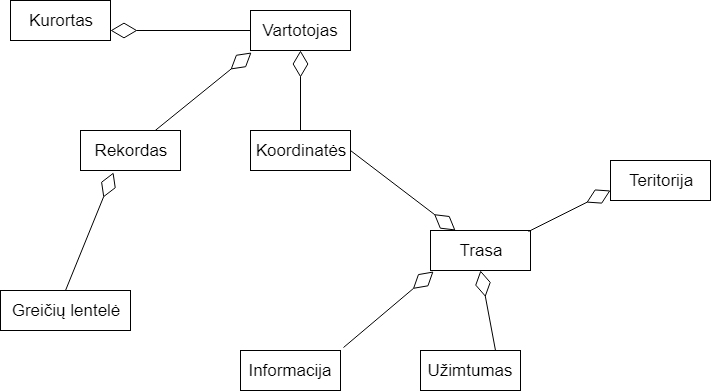
\includegraphics[width=18cm,height=20cm,keepaspectratio]{DomainModel.png}
	\caption{Domain model}
	\label{fig:Domain model}
\end{figure}
\begin{figure}[H]
		\centering	
	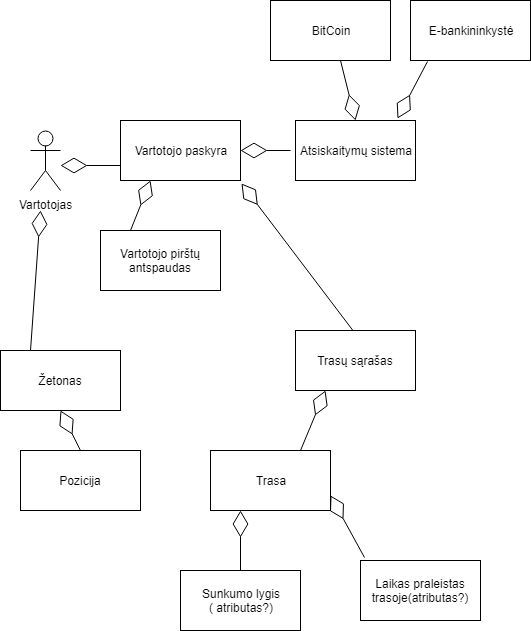
\includegraphics[width=18cm,height=20cm,keepaspectratio]{Domain2.png}
	\caption{Domain model}
	\label{fig:Domain model}
\end{figure}
Sudarius domain modelio drafta galime pradėti braižyti use case diagramą ir GUI darftini variantą. Ne viskas kas bus use case diagramoje yra domanin model diagramoje bet vėliau jis bus papildytas.



Use case draftas

\begin{figure}[H]
		\centering	
	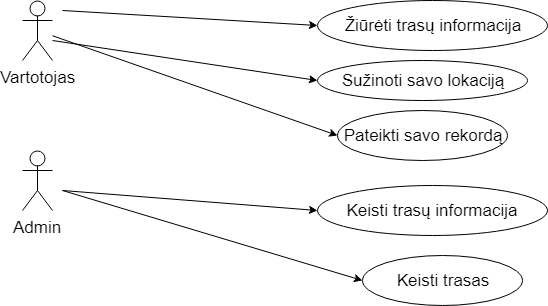
\includegraphics[width=18cm,height=20cm,keepaspectratio]{UseCase.png}
	\caption{Use case}
	\label{fig:Use case}
\end{figure}

\begin{table}[htbp]

\begin{tabularx}{1\textwidth}{ |P{17cm}|}  \hline

Pagrindinis scenarijus \\ \hline
Vartotojas prisijungia prie savo paskyros ir paspaudžia mygtuką ,,Atsiskaityti už paslaugas". Sistema pateikia pasirinkimą mokėti per E-bankininkystę arba BitCoin pervedimu. Vartotojas pasirenka norimą pasirinkimą \\ \hline
Alternatyvus scenarijus \\ \hline
Vartotojas pasirenka norimą apmokėjimo būdą, tačiau pasirinkas apmokėjimo būdas nėra pasiekiams. Vartotojui parodoma informacinę žinutę apie nepasiekiamą galimybė ir jis nukreipiamas atgal į apmokėjimo langą \\ \hline





\end{tabularx}

	
\end{table}



GUI draftas
\begin{figure}[H]
		\centering	
	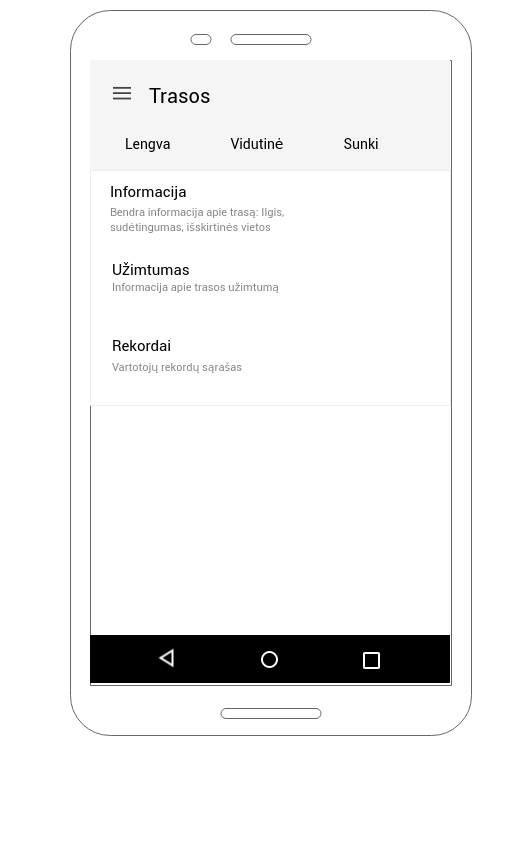
\includegraphics[width=18cm,height=20cm,keepaspectratio]{GUI.png}
	\caption{GUI}
	\label{fig:GUI}
\end{figure}









 
	

\section{Užduotys}

\section{Reikalavimų specifikacijos, dalykinės srities modelio ir užduočių diagramos peržiūros rezultatai}

\section{Išvada}

\section{Asmeninis darbo indėlis}

\section{Žodynas}


	
	





\end{document}